% !TEX encoding = UTF-8 Unicode

% Based on https://github.com/Miracle0565/BUCT-Beamer-Theme

\documentclass[
10pt,  
aspectratio=43,  
]{beamer}
\setbeamercovered{transparent=10}
\usetheme[
%  showheader,  
%  red,  
  purple,  
%  gray,  
%  graytitle,  
  colorblocks,  
%  noframetitlerule,  
]{Verona}

\usepackage[T1]{fontenc}
\usepackage{tikz}
\usepackage[utf8]{inputenc}
\usepackage{lipsum}
%%%%%%%%%%%%%%%%%%%%%%%%%%%%%%%
% Mac上使用如下命令声明隶书字体,  windows也有相关方式,  大家可自行修改
\providecommand{\lishu}{\CJKfamily{zhli}}
%%%%%%%%%%%%%%%%%%%%%%%%%%%%%%%
\usepackage{tikz}
\usetikzlibrary{fadings}
%
%\setbeamertemplate{sections/subsections in toc}[ball]
\usepackage{xeCJK}
\usepackage{listings}
\usepackage{caption}
\usepackage{subfigure}
\usefonttheme{professionalfonts}
\def\mathfamilydefault{\rmdefault}
\usepackage{amsmath}
\usepackage{multirow}
\usepackage{booktabs}
\usepackage{bm}
\setbeamertemplate{section in toc}{\hspace*{1em}\inserttocsectionnumber.~\inserttocsection\par}
\setbeamertemplate{subsection in toc}{\hspace*{2em}\inserttocsectionnumber.\inserttocsubsectionnumber.~\inserttocsubsection\par}
\setbeamerfont{subsection in toc}{size=\small}
\AtBeginSection[]{%
	\begin{frame}%
		\frametitle{Outline}%
		\textbf{\tableofcontents[currentsection]} %
	\end{frame}%
}

\AtBeginSubsection[]{%
	\begin{frame}%
		\frametitle{Outline}%
		\textbf{\tableofcontents[currentsection,   currentsubsection]} %
	\end{frame}%
}

\title{高等数学C}
%\subtitle{A Simple while elegant template}
\author[P.Yu]{余沛}
\mail{peiy\_gzgs@qq.com}
\institute[Guangzhou College of Technology and Business]{Guangzhou College of Technology and Business \\
  广州工商学院}
\date{\today}
\titlegraphic[width=4cm]{logo.png}{}




%%%%%%%%%%%%%%%%%%%%%%%%%%%%%%%%
% ----------- 标题页 ------------
%%%%%%%%%%%%%%%%%%%%%%%%%%%%%%%%



\begin{document}

\maketitle

%%% define code
\defverbatim[colored]\lstI{
	\begin{lstlisting}[language=C++,  basicstyle=\ttfamily,  keywordstyle=\color{red}]
	int main() {
	// Define variables at the beginning
	// of the block,   as in C: 
	CStash intStash,   stringStash;
	int i;
	char* cp;
	ifstream in;
	string line;
	[...]
	\end{lstlisting}
}
%%%%%%%%%%%%%%%%%%%%%%%%%%%%%%%%
% ----------- FRAME ------------
%%%%%%%%%%%%%%%%%%%%%%%%%%%%%%%%

\section{极限的运算法则}
\subsection{回顾: 数列极限,  函数极限,  无穷小量,  无穷大量}

\begin{frame}[c]{极限的定义}
	\begin{columns}[onlytextwidth]
		\column{0.4\textwidth}
		
		\begin{block}{定义: 数列极限与收敛数列的定义}
			对于数列 $\{x_n\}$ 和常数 $a$,  如果有: 对于任意的 $\epsilon>0$,  都存在正整数 $N$,  使得对于任意满足 $n>N$ 的 $n$,  不等式
			$$|x_n-a|<\epsilon$$
			都成立,  
			那么称常数 $a$ 是数列 $\{x_n\}$ 的极限,  或者数列 $\{x_n\}$ \textbf{收敛},  并且收敛于 $a$,  记为
			\begin{equation*}
				\lim_{n\to\infty}x_n=a,   \quad 
			\end{equation*}
			\begin{equation*}
				x_n\to a (n\to\infty).
			\end{equation*}
		\end{block}
		\column{0.5\textwidth}
		
		\begin{figure}
			\flushleft 
			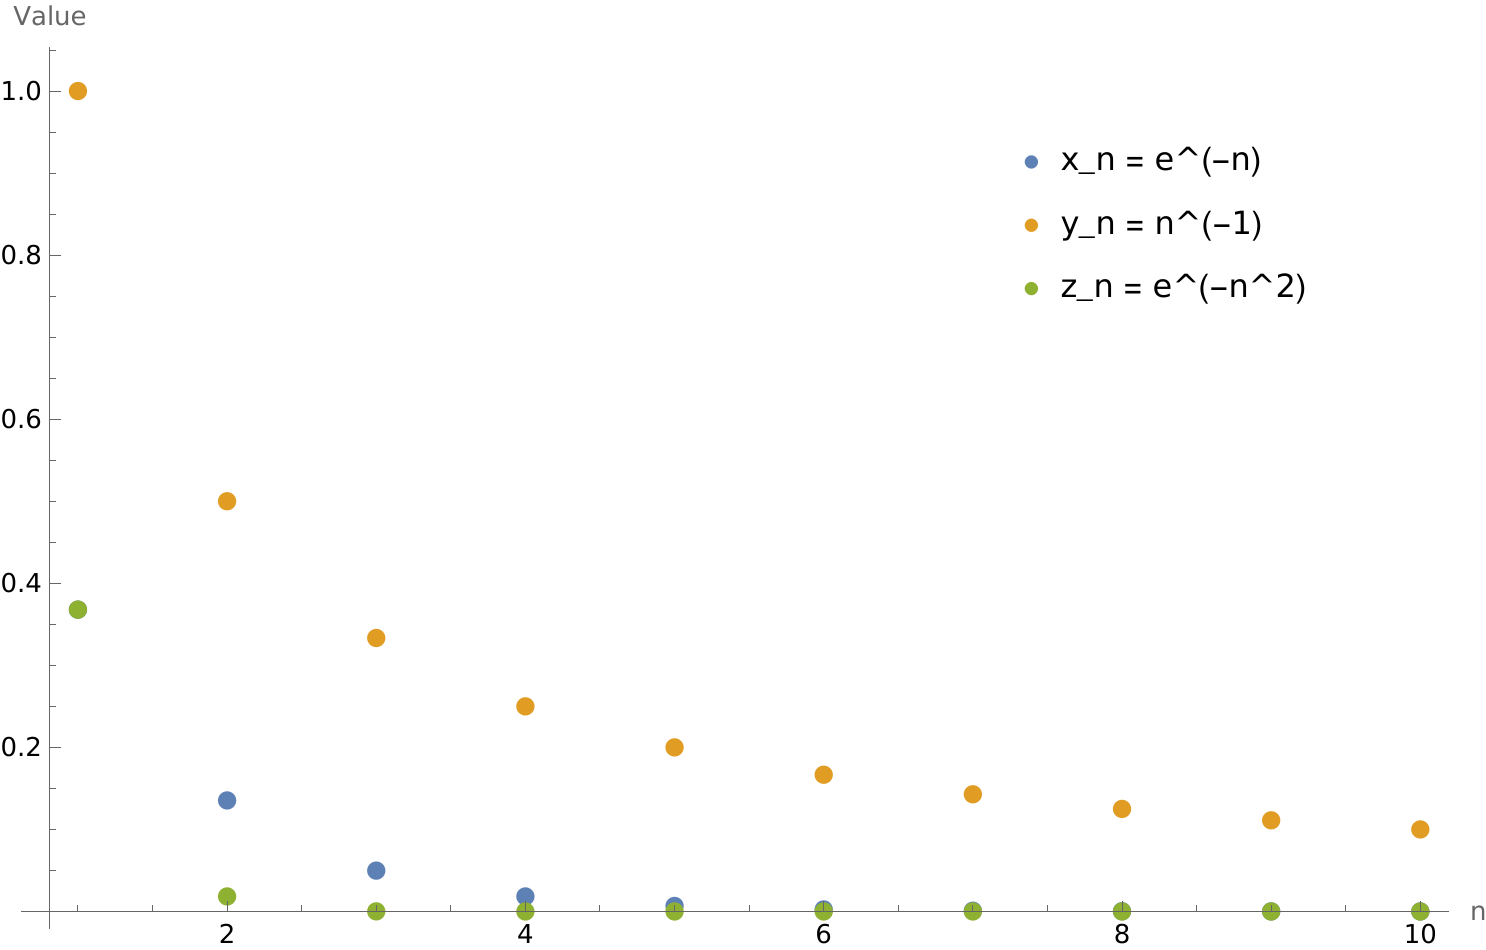
\includegraphics[width=1\linewidth]{convergent series1.png}
			\caption{三种收敛数列}
			
		\end{figure}
	\end{columns}
\end{frame}	

\begin{frame}[c]{极限的定义}
	\begin{columns}[onlytextwidth]
		\column{0.4\textwidth}
		
		\begin{block}{函数极限的数列定义}
			设函数 $f(x)$ 在点 $x=a$ 的某个去心邻域内有定义,  如果存在常数 $L$,  对于任意定义在该去心邻域上收敛到$a$的数列 $\{x_n\}$,  都有 
			\begin{equation*}
				\lim_{n\to\infty} f(x_n)` = L,  
			\end{equation*}
			则称函数 $f(x)$ 在 $x=a$ 处\textbf{收敛}于 $L$,  记作 $\lim_{x \to a} f(x) = L$.
		\end{block}
		\column{0.6\textwidth}
		
		
		\begin{figure}
			\centering
			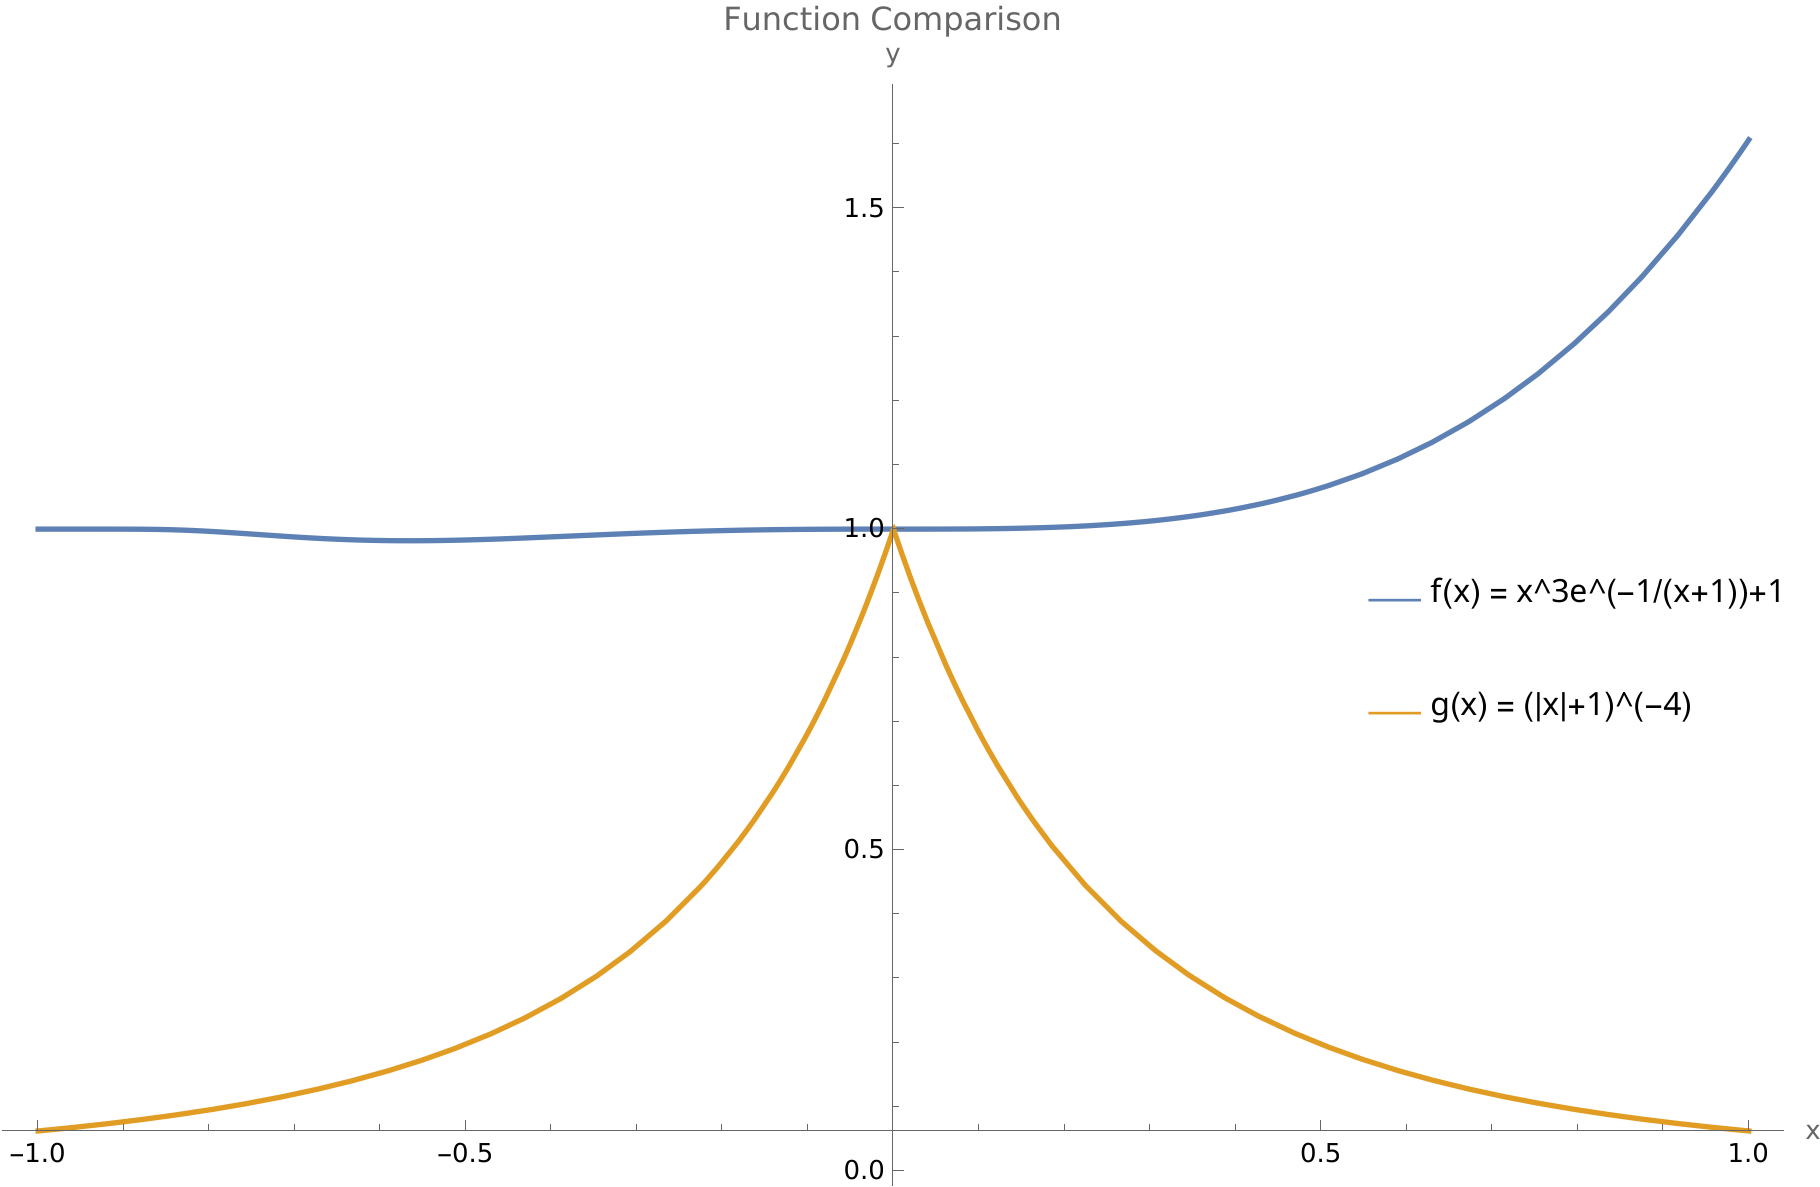
\includegraphics[width=0.9\linewidth]{convergent function1.png}
			\caption{两种在$x=0$处收敛的函数}
			
		\end{figure}
	\end{columns}
\end{frame}	

\begin{frame}[c]{无穷小量与无穷大量}
		
	\begin{columns}[onlytextwidth]
		\column{0.4\textwidth}
		\begin{block}{定义: 无穷小量}设函数 $f(x)$ 在 $x=a$ 处有定义,  如果对于任意给定的正数 $\varepsilon$,  存在正数 $\delta$,  使得当 $0 < |x-a| < \delta$ 时,  有 $|f(x)| < \varepsilon$,  则称函数 $f(x)$ 在 $x=a$ 处为无穷小量,  记为
			\begin{equation*}
				\lim_{x\to a}f(x) = 0.
			\end{equation*}
		\end{block}
		
		\column{0.6\textwidth}
		\begin{figure}
			\centering
			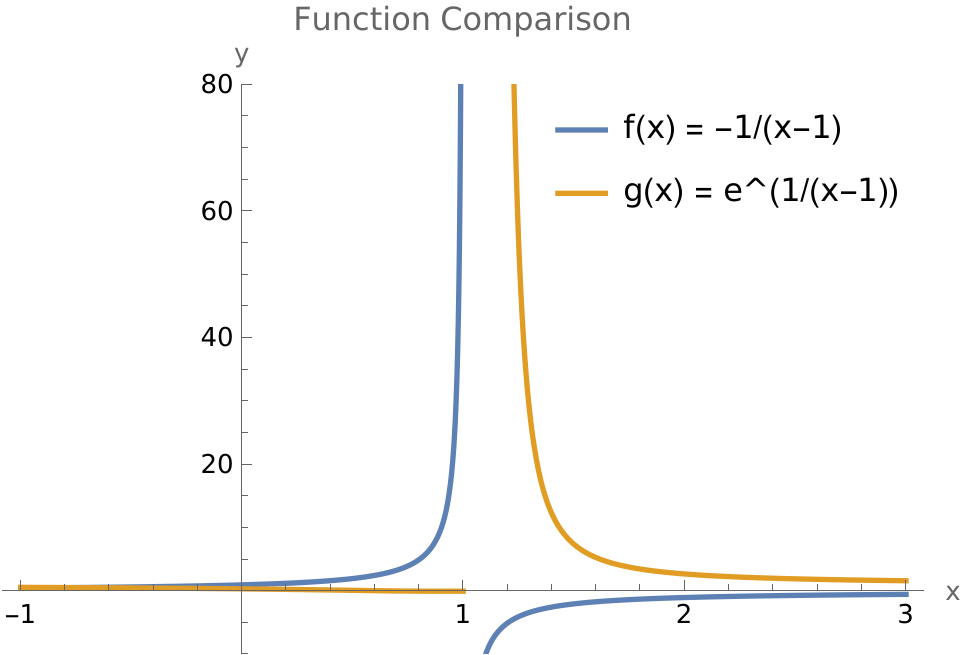
\includegraphics[width=0.8\linewidth]{infinity2.png}
			
		\end{figure}
	\end{columns}
\end{frame}	


\begin{frame}[c]{无穷小量与无穷大量}
		
	\begin{columns}[onlytextwidth]
		\column{0.4\textwidth}
		
		
		\begin{block}{定义: 无穷大量}设函数 $f(x)$ 在 $x=a$ 处有定义,  如果对于任意给定的正数 $M$,  存在正数 $\delta$,  使得当 $0 < |x-a| < \delta$ 时,  有 $|f(x)| > M$,  则称函数 $f(x)$ 在 $x=a$ 处为无穷大量,  记为
			\begin{equation*}
				\lim_{x\to a}f(x) = \infty.
			\end{equation*}
		\end{block}
		\begin{exampleblock}{注意}
			注意分辨 $-\infty$,   $+\infty$ 和 $\infty$.
		\end{exampleblock}
		\column{0.6\textwidth}
		\begin{figure}
			\centering
			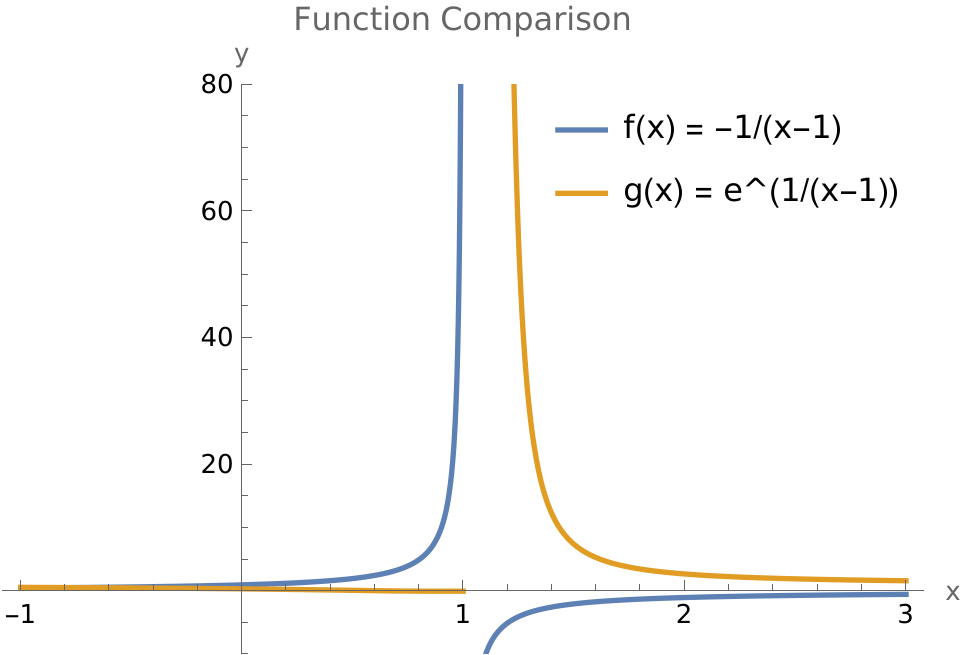
\includegraphics[width=0.8\linewidth]{infinity2.png}
			
		\end{figure}
	\end{columns}
\end{frame}	




\subsection{回顾: 极限的基本运算}
\begin{frame}[c]{极限的基本运算: 四则运算}
	\begin{block}{极限的四则运算}
		对于 $x_0,  A,  B,  k \in \mathbb{R}$,  如果有 $\lim _{\substack{x \rightarrow x_0 \\(x \rightarrow \pm\infty)}} f(x)=A$ 和 $ \lim _{\substack{x \rightarrow x_0 \\(x \rightarrow \pm\infty)}} g(x)=B$,   则有: 
		\pause
		
		\begin{enumerate}
			\item $\lim _{\substack{x \rightarrow x_0 \\(x \rightarrow \pm\infty)}}[f(x) \pm g(x)]=A \pm B$,  \\
			      \pause
			\item
			      $\lim _{\substack{x \rightarrow x_0 \\(x \rightarrow \pm\infty)}}[k f(x)]=k A$,  \\
			      \pause
			\item $\lim _{\substack{x \rightarrow x_0 \\(x \rightarrow\pm \infty)}}[f(x) \cdot g(x)]=A B$,  \\
			      \pause
			\item $\lim _{\substack{x \rightarrow x_0 \\(x \rightarrow\pm \infty)}} \displaystyle\frac{f(x)}{g(x)}=\frac{A}{B} \quad(B \neq 0)$.
		\end{enumerate}
	\end{block}
	\begin{exampleblock}{注意}
		注意这些运算的复合形式.
	\end{exampleblock}
\end{frame}

\subsection{算例}
\begin{frame}
	\frametitle{多项式的情形}
	\begin{block}{多项式函数 $P_n(x)$}
		记多项式函数为 $P_n(x) : = a_n x^n+a_{n-1} x^{n-1}+\cdots+a_{1} x+a_0$.
	\end{block}
	\begin{exampleblock}{情形一}
		一般地,   用极限四则运算法则可得到
		$$
		\lim _{x \rightarrow x_0}a_n x^n+a_{n-1} x^{n-1}+\cdots+a_{1} x+a_0=a_n x_0^n+a_{n-1} x^{n-1}+\cdots+a_{1} x_0+a_n.
		$$
		即
		$$
		\lim _{x \rightarrow x_0}P_n(x)=P_n(x_0).
		$$
	\end{exampleblock}
	
\end{frame}

\begin{frame}
	\frametitle{多项式的情形}
	
	\begin{exampleblock}{情形二}
		记$R(x)=\displaystyle\frac{p_n(x)}{q_m(x)}$,   其中 $p_n(x),   q_m(x)$ 分别是 $n$ 次和 $m$ 次多项式函数(此时 也称 $R(x)$ 为有理函数),  且 $q_m\left(x_0\right) \neq 0$,   则
		$$\lim _{x \rightarrow x_0} R(x)=R\left(x_0\right)=\frac{p_n\left(x_0\right)}{q_m\left(x_0\right)}.$$
	\end{exampleblock}
	例:  求 $$\lim _{x \rightarrow 1} \frac{x^3+2 x^2+4 x+1}{3 x^4+x^3-2 x^2+4 x+2}.$$
	
\end{frame}

\begin{frame}
	\frametitle{多项式的情形}
	
	\begin{exampleblock}{情形三}
		$$
		\lim _{x \rightarrow \infty} \frac{a_k x^k+a_{k-1} x^{k-1}+\cdots+a_0}{b_l x^{l}+b_{l-1} x^{l-1}+\cdots+b_0}=\left\{\begin{array}{cc}
		0 & k<l,   \\
		\displaystyle\frac{a_k}{b_l} & k=l,   \\
		\infty & k>l.
		\end{array}\right.
		$$
	\end{exampleblock}
	例:  求 $$\displaystyle\lim_{x \rightarrow \infty} \frac{3 x^2-2 x+1}{-2 x^2+x-4}.$$
\end{frame}

\subsection{复合函数极限}

\begin{frame}
	\frametitle{定理: 复合函数的极限}
	
	\begin{block}{复合函数的极限}
		如果 $y=f(u)$ 与 $u=\varphi(x)$ 构成复合函数$y=f(\varphi(x))$. 若 $\lim _{u \rightarrow u_0} f(u)=a$,   $\lim _{x \rightarrow x_0} \varphi(x)=u_0$,   则有 $\lim _{x \rightarrow x_0} f(\varphi(x))=\lim _{u \rightarrow u_0} f(u)=a$.
	\end{block}
	\pause
	\begin{exampleblock}{补充推论: 幂指函数的极限}
		设 $\lim f(x)=a(a>0),   \lim g(x)=b$,   则有
		$$
		\operatorname{limf}(x)^{g(x)}=[\lim f(x)]^{\lim g(x)}=a^b.
		$$
	\end{exampleblock}
\end{frame}


\subsection{三明治法则和单调有界法则}

\begin{frame}
	\frametitle{极限的三明治法则}
	
	\begin{block}{定理: 极限的三明治法则}
		设函数 $f(x)$,   $g(x)$ 和 $h(x)$ 满足以下条件: 
		\begin{itemize}
			\item 对于 $a$ 的某个邻域中的所有 $x$,  有 $g(x) \leq f(x) \leq h(x)$;
			\item 当 $g(x)\to L$$(x\to a)$ 和 $g(x)\to L$$(x\to a)$ 同时成立.
		\end{itemize}
		则当 $x$ 趋近于 $a$ 时,  $f(x)$ 也趋近于 $L$.
	\end{block}
	
	\begin{exampleblock}{例子}
		考虑函数 $f(x) = x^2 \sin\left(\frac{1}{x}\right)$,  我们想要计算 $\lim_{x \to 0} f(x)$.我们可以使用夹逼定理来求解.
		
		首先,  我们可以证明对于所有 $x$,  有 $-x^2 \leq f(x) \leq x^2$.其次,  当 $x$ 趋近于 $0$ 时,  $-x^2$ 和 $x^2$ 都趋近于 $0$.因此,  根据夹逼定理,  $\lim_{x \to 0} f(x) = 0$.
	\end{exampleblock}
	
\end{frame}

\begin{frame}
	\frametitle{极限的三明治法则}
	
	\begin{figure}
		\centering
		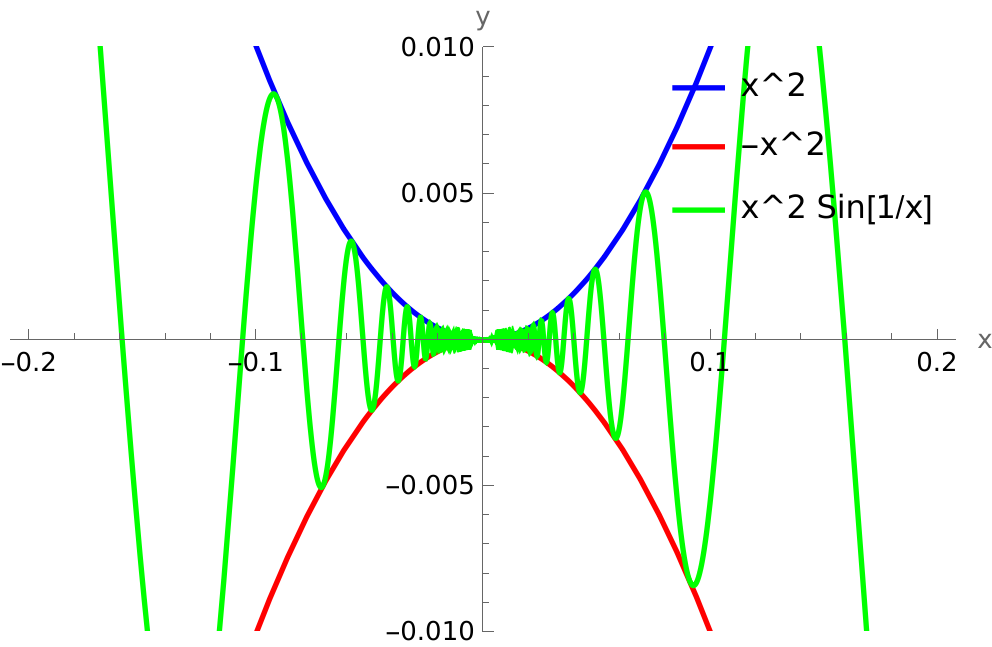
\includegraphics[width=1\linewidth]{sandwich.png}
		
		
	\end{figure}
\end{frame}

\begin{frame}
	\frametitle{单调收敛法则}
	\begin{block}{定理}
		单调有界数列收敛.
	\end{block}
	
\end{frame}

\section{两个重要极限}
\subsection{$\lim_{x\to0}\frac{\sin(x)}{x}$}

\begin{frame}
	\frametitle{$\lim_{x\to0}\frac{\sin(x)}{x}$}
	\begin{block}{结论}
		$$
		\lim _{x \rightarrow 0} \frac{\sin x}{x}=1.
		$$
	\end{block}
	原因: 回顾割圆术.
	
	\begin{exampleblock}{例子}
		求:  $$\displaystyle\lim _{x \rightarrow 0} \frac{\tan x}{x},   \lim_{x \rightarrow 0} \frac{\sin k x}{x},   \lim _{x\rightarrow 0} \frac{1-\cos x}{x^2}$$.
	\end{exampleblock}
	
\end{frame}

\subsection{$\lim_{n\to\infty}\left(1+\frac1x\right)^x$}

\begin{frame}
	\frametitle{$\lim_{n\to\infty}\left(1+\frac1x\right)^x$}
	\begin{block}{结论}
		$$
		\lim _{x \rightarrow \infty}\left(1+\frac{1}{x}\right)^x=e.
		$$
	\end{block}
	原因: 考虑自然对数的增长率问题: 
	\begin{equation*}
		\begin{aligned}
			\lim _{h \rightarrow 0} \frac{\log _a(x+h)-\log _a(x)}{h} & =\lim _{h \rightarrow 0} \frac{\log _a(1+h / x)}{x \cdot h / x}             \\
			                                                          & =\frac{1}{x} \log _a\left(\lim _{u \rightarrow 0}(1+u)^{\frac{1}{u}}\right) \\
			                                                          & =\frac{1}{x} \log _a e,                                                     
		\end{aligned}
	\end{equation*}
\end{frame}

\begin{frame}
	\frametitle{$\lim_{n\to\infty}\left(1+\frac1x\right)^x$}
	\begin{exampleblock}{例子}
		求: $$
		\lim _{x \rightarrow \infty}\left(1+\frac{4}{x}\right)^x,   \lim _{x \rightarrow 0}\left(1-\frac{2}{x}\right)^x.
		$$
	\end{exampleblock}
	
	\begin{equation*}
		\begin{aligned}
			\lim _{x \rightarrow 0}\left(1+\frac{4}{x}\right)^x=\lim _{x \rightarrow 0}\left[1+\left(-\frac{2}{x}\right)\right]^{\frac{4x}{4}}=e^{4}, 
		\end{aligned}
	\end{equation*}
	
	
	\begin{equation*}
		\begin{aligned}
			\lim _{x \rightarrow 0}\left(1-\frac{2}{x}\right)^x=\lim _{x \rightarrow 0}\left[1+\left(-\frac{2}{x}\right)\right]^{\frac{x}{-2}} \cdot(-2)=e^{-2}. 
		\end{aligned}
	\end{equation*}
\end{frame}

% Thank you page
\beamertemplateshadingbackground{structure.fg!90}{structure.fg}
\begin{frame}[plain]
	\vfill
	\centering
	{
		\centering \Huge \color{white} Thank you for your attention!\\[10pt]Questions?\\Homework: Page79:  11(1)—(8),   Page81:  23、24
	}
	\vfill
\end{frame}


\end{document}

